% !TEX encoding = UTF-8 Unicode
\documentclass[aspectratio=169, 10pt]{beamer}

% Пакеты для русского языка
\usepackage[T2A]{fontenc}
\usepackage[utf8]{inputenc}
\usepackage[russian]{babel}

% Пакеты для математики
\usepackage{amsmath}
\usepackage{amssymb}
\usepackage{mathtools}

% Пакеты для графики
\usepackage{graphicx}
\usepackage{tikz}
\usetikzlibrary{arrows.meta, positioning, shapes, calc}

% Пакеты для таблиц
\usepackage{booktabs}
\usepackage{array}

% Настройка темы
\usetheme{Madrid}
\usecolortheme{seahorse}

% Настройка цветов
\definecolor{primary}{RGB}{15, 76, 129}
\definecolor{secondary}{RGB}{46, 117, 182}
\definecolor{accent}{RGB}{214, 228, 240}

\setbeamercolor{structure}{fg=primary}
\setbeamercolor{title}{fg=white, bg=primary}
\setbeamercolor{frametitle}{fg=white, bg=primary}
\setbeamercolor{block title}{bg=secondary, fg=white}
\setbeamercolor{block body}{bg=accent}

% Уменьшенные настройки шрифтов
\setbeamerfont{title}{size=\large, series=\bfseries}
\setbeamerfont{subtitle}{size=\small}
\setbeamerfont{frametitle}{size=\normalsize, series=\bfseries}
\setbeamerfont{framesubtitle}{size=\small}
\setbeamerfont{block title}{size=\small, series=\bfseries}
\setbeamerfont{normal text}{size=\footnotesize}
\setbeamerfont{itemize/enumerate body}{size=\footnotesize}
\setbeamerfont{itemize/enumerate subbody}{size=\scriptsize}

% Настройка расстояний
\setbeamersize{text margin left=0.6cm, text margin right=0.6cm}
\setlength{\columnsep}{15pt}  % Расстояние между колонками

% Удаление навигации
\setbeamertemplate{navigation symbols}{}

% Название презентации
\title{Рекуррентные нейронные сети}
\subtitle{Математические основы и применения}
\author{}
\date{}

\begin{document}

% Слайд 1: Титульный
\begin{frame}[plain]
  \titlepage
\end{frame}

% Слайд 2: Что такое RNN
\begin{frame}{Что такое RNN?}
  \begin{columns}[T]
    \begin{column}{0.45\textwidth}
      \begin{block}{Определение}
        \textbf{RNN} — класс нейронных сетей для обработки \textbf{последовательных данных}
      \end{block}
      
      \vspace{0.2cm}
      
      \begin{block}{Ключевые особенности}
        \begin{itemize}
          \item \textbf{Внутренняя память} — $h_t$           \item \textbf{Разделяемые веса}
          \item Обработка произвольной длины
        \end{itemize}
      \end{block}
    \end{column}
    
    \begin{column}{0.45\textwidth}
      \begin{block}{Примеры данных}
        \begin{itemize}
          \item Тексты (слова)
          \item Речь (аудио)
          \item Временные ряды
          \item Видео (кадры)
          \item ДНК
        \end{itemize}
      \end{block}
    \end{column}
  \end{columns}
\end{frame}

% Слайд 3: Проблема обработки последовательностей
\begin{frame}{Проблема обработки последовательностей}
  \begin{columns}[T]
    \begin{column}{0.45\textwidth}
      \begin{block}{Стандартные нейросети}
        \textbf{Ограничения:}
        \begin{itemize}
          \item Фиксированный размер входа
          \item Нет памяти
          \item Разные веса
          \item Не учитывают контекст
        \end{itemize}
      \end{block}
    \end{column}
    
    \begin{column}{0.45\textwidth}
      \begin{block}{RNN}
        \textbf{Преимущества:}
        \begin{itemize}
          \item Переменная длина
          \item Внутреннее состояние
          \item Разделяемые веса $W$, $b$           \item Учитывают контекст
        \end{itemize}
      \end{block}
    \end{column}
  \end{columns}
\end{frame}

% Слайд 4: Архитектура ячейки RNN
\begin{frame}{Архитектура ячейки RNN}
  \begin{columns}[T]
    \begin{column}{0.5\textwidth}
      \centering
      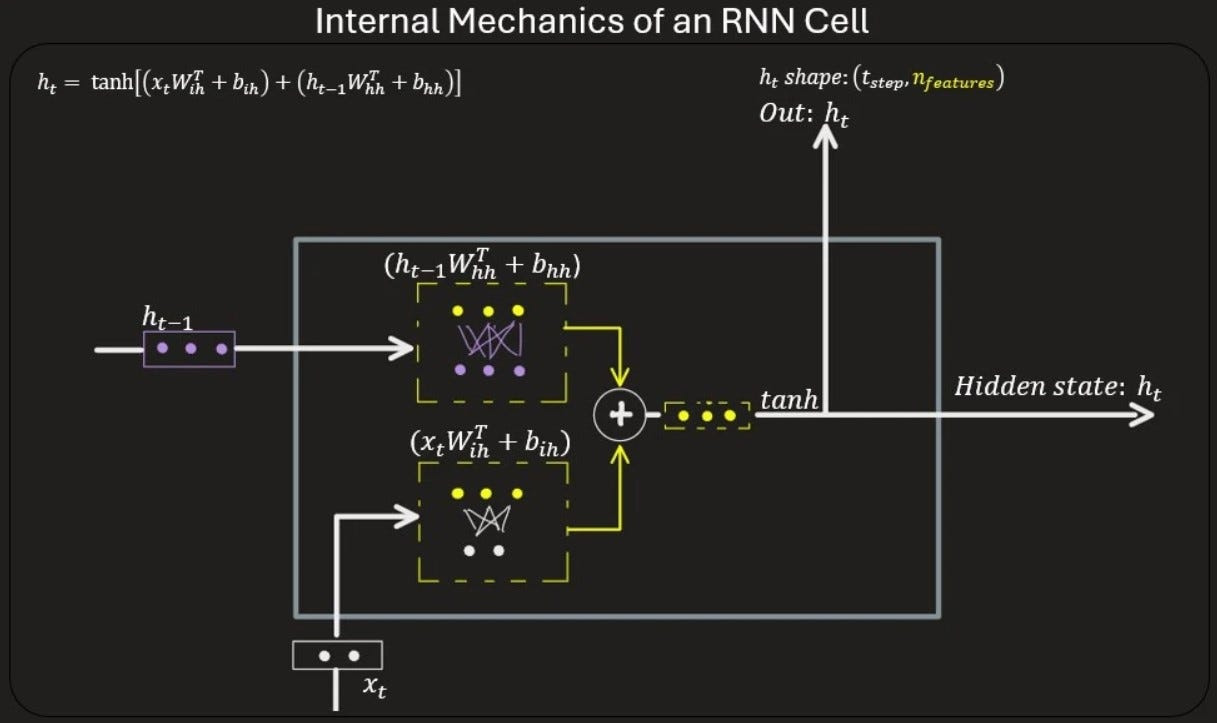
\includegraphics[width=0.85\textwidth]{images/rnn_cell.jpeg}
    \end{column}
    
    \begin{column}{0.42\textwidth}
      \begin{block}{Компоненты}
        \textbf{Входы:}
        \begin{itemize}
          \item $x_t$ — текущий вход
          \item $h_{t-1}$ — прошл. состояние
        \end{itemize}
        
        \textbf{Параметры:}
        \begin{itemize}
          \item $W_{xh}$, $W_{hh}$ — веса
          \item $b_h$ — смещение
        \end{itemize}
        
        \textbf{Выход:}
        \begin{itemize}
          \item $h_t$ — новое состояние
        \end{itemize}
      \end{block}
    \end{column}
  \end{columns}
\end{frame}

% Слайд 5: Математика базовой RNN
\begin{frame}{Математика базовой RNN}
  \begin{columns}[T]
    \begin{column}{0.48\textwidth}
      \centering
      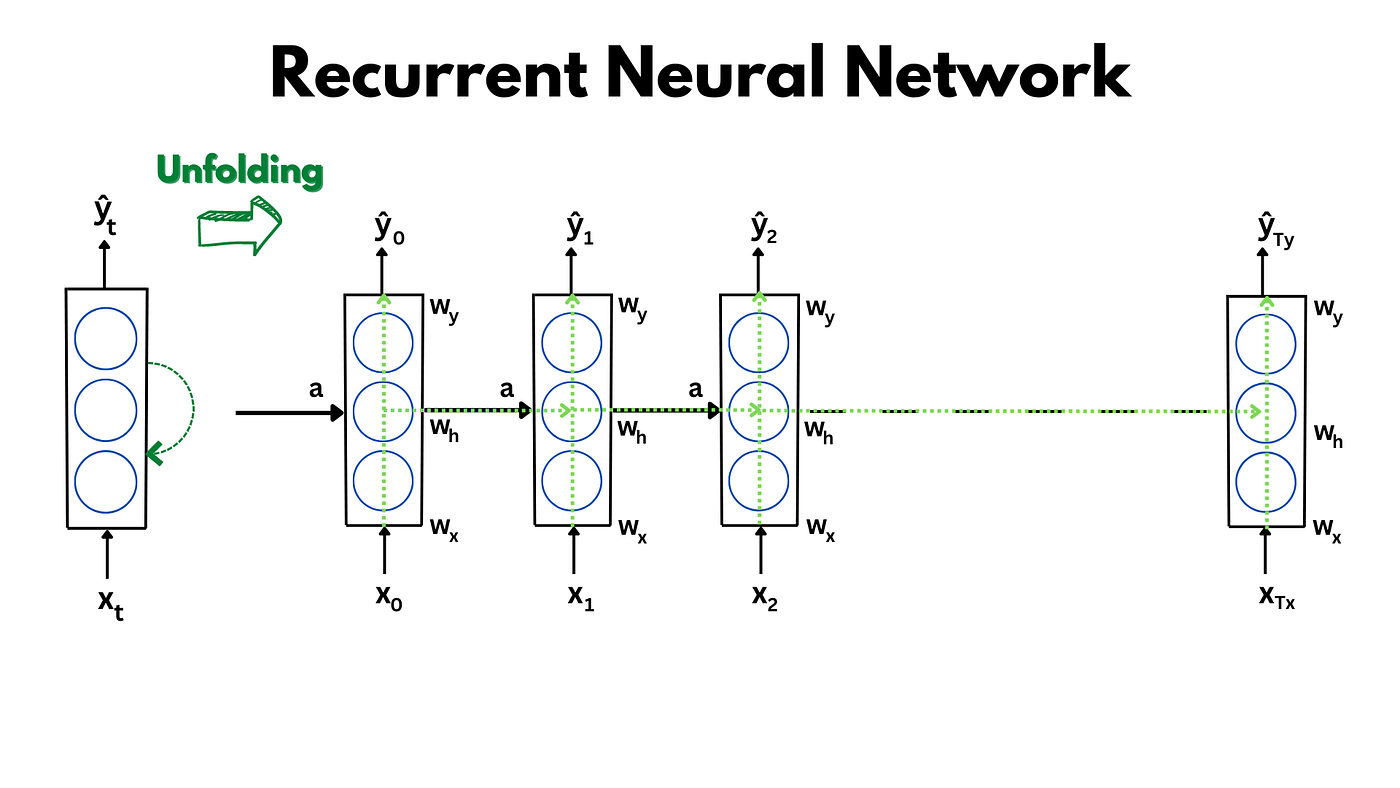
\includegraphics[width=0.85\textwidth]{images/rnn_unrolled.png}
    \end{column}
    
    \begin{column}{0.44\textwidth}
      \begin{block}{Формулы Vanilla RNN}
        \textbf{Скрытое состояние:}
        \[
          h_t = \tanh(W_{xh} x_t + W_{hh} h_{t-1} + b_h)
        \]
        
        \textbf{Выход:}
        \[
          y_t = W_{hy} h_t + b_y
        \]
      \end{block}
      
      \begin{alertblock}{Ключевая особенность}
        Параметры $W$, $b$ \textbf{разделяются} на всех шагах.
      \end{alertblock}
    \end{column}
  \end{columns}
\end{frame}

% Слайд 6: Развертывание сети во времени
\begin{frame}{Развертывание сети во времени}
  \begin{block}{Концепция}
    RNN разворачивается во времени — каждый шаг обрабатывается отдельной копией с \textbf{одинаковыми весами}.
  \end{block}
  
  \centering
  \vspace{0.2cm}
  \begin{tikzpicture}[
    node distance=1.0cm,
    block/.style={rectangle, draw, fill=primary!20, minimum width=0.9cm, minimum height=0.7cm, align=center, font=\scriptsize},
    arrow/.style={-{Stealth}, thick}
  ]
    \node[block] (h0) {$h_0$};
    \node[block, right=of h0] (h1) {$h_1$};
    \node[block, right=of h1] (h2) {$h_2$};
    \node[block, right=of h2] (h3) {$h_3$};
    
    \node[block, below=of h1] (x1) {$x_1$};
    \node[block, below=of h2] (x2) {$x_2$};
    \node[block, below=of h3] (x3) {$x_3$};
    
    \node[block, above=of h1] (y1) {$y_1$};
    \node[block, above=of h2] (y2) {$y_2$};
    \node[block, above=of h3] (y3) {$y_3$};
    
    \draw[arrow] (h0) -- (h1);
    \draw[arrow] (h1) -- (h2);
    \draw[arrow] (h2) -- (h3);
    
    \draw[arrow] (x1) -- (h1);
    \draw[arrow] (x2) -- (h2);
    \draw[arrow] (x3) -- (h3);
    
    \draw[arrow] (h1) -- (y1);
    \draw[arrow] (h2) -- (y2);
    \draw[arrow] (h3) -- (y3);
    
    \node[below=1.2cm of h2, font=\scriptsize] {$W$, $b$ — shared weights};
  \end{tikzpicture}
\end{frame}

% Слайд 7: Обучение RNN (BPTT)
\begin{frame}{Обучение: Backpropagation Through Time}
  \begin{block}{Алгоритм BPTT}
    \begin{enumerate}
      \item \textbf{Forward Pass:} Обработка шаг за шагом
      \item \textbf{Loss:} Вычисление ошибки $L = \sum_{t=1}^{T} L_t$       \item \textbf{Backward:} Обратное распространение от $T$ к $1$       \item \textbf{Update:} Обновление весов по сумме градиентов
    \end{enumerate}
  \end{block}
  
  \vspace{0.2cm}
  
  \begin{block}{Правило цепочки}
    \[
      \frac{\partial L}{\partial W} = \sum_{t=1}^{T} \frac{\partial L_t}{\partial h_t} \cdot \frac{\partial h_t}{\partial h_{t-1}} \cdot \frac{\partial h_{t-1}}{\partial W}
    \]
  \end{block}
  
  \begin{alertblock}{Truncated BPTT}
    Для длинных последовательностей: window size $k \approx 20-50$.
  \end{alertblock}
\end{frame}

% Слайд 8: Проблема исчезающего градиента
\begin{frame}{Проблема исчезающего градиента}
  \begin{block}{Математическая причина}
    \[
      \frac{\partial h_t}{\partial h_j} = \prod_{k=j+1}^{t} W_{hh}^{T} \cdot \text{diag}(f'(z_k))
    \]
  \end{block}
  
  \vspace{0.2cm}
  
  \begin{columns}[T]
    \begin{column}{0.45\textwidth}
      \begin{alertblock}{Условие}
        Если $\max |\lambda(W_{hh})| < 1$:
        \[
          \left\| \frac{\partial h_t}{\partial h_j} \right\| \to 0
        \]
      \end{alertblock}
    \end{column}
    
    \begin{column}{0.45\textwidth}
      \begin{alertblock}{Последствия}
        \begin{itemize}
          \item Градиенты исчезают
          \item Веса не обновляются
          \item Забывает контекст
        \end{itemize}
      \end{alertblock}
    \end{column}
  \end{columns}
\end{frame}

% Слайд 9: Проблема взрывающегося градиента
\begin{frame}{Проблема взрывающегося градиента}
  \begin{columns}[T]
    \begin{column}{0.45\textwidth}
      \begin{alertblock}{Взрывающийся градиент}
        \textbf{Причина:} $\max |\lambda(W_{hh})| > 1$         
        \[
          \left\| \nabla h_t \right\| \propto \lambda^{t}
        \]
        
        \textbf{Последствия:}
        \begin{itemize}
          \item NaN
          \item Нестабильно
          \item Резкие изменения
        \end{itemize}
      \end{alertblock}
    \end{column}
    
    \begin{column}{0.45\textwidth}
      \begin{exampleblock}{Gradient Clipping}
        \textbf{Алгоритм:}
        \begin{enumerate}
          \item Градиент $g$           \item Если $\|g\| > threshold$:
          \[
            g = \text{threshold} \cdot \frac{g}{\|g\|}
          \]
          \item $W = W - \eta g$         \end{enumerate}
        
        threshold $\in [1, 5]$       \end{exampleblock}
    \end{column}
  \end{columns}
\end{frame}

% Слайд 10: Введение в LSTM
\begin{frame}{Долгая краткосрочная память (LSTM)}
  \begin{columns}[T]
    \begin{column}{0.52\textwidth}
      \centering
      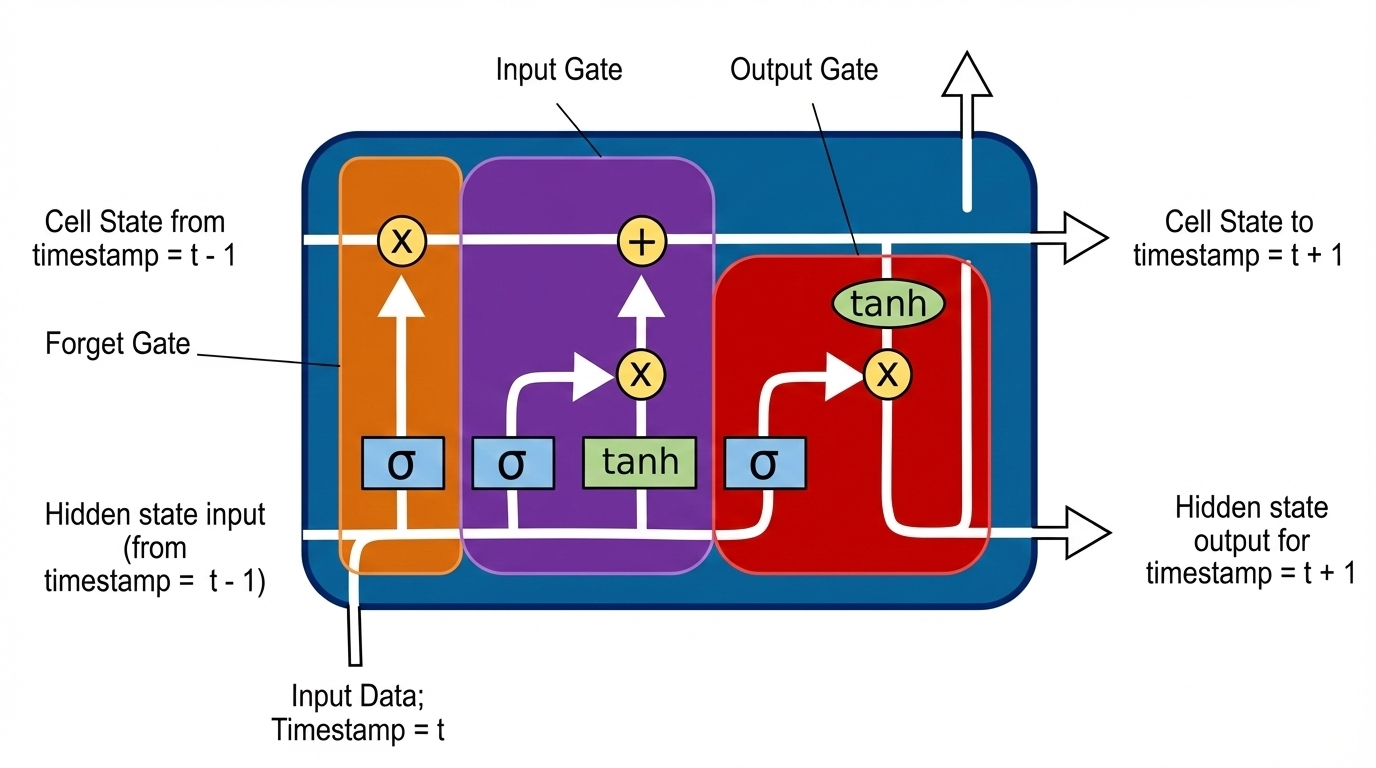
\includegraphics[width=0.85\textwidth]{images/lstm_architecture.png}
    \end{column}
    
    \begin{column}{0.42\textwidth}
      \begin{block}{Компоненты}
        \textbf{Cell State} ($C_t$):
        \begin{itemize}
          \item Конвейер информации
          \item Прямой поток градиента
        \end{itemize}
        
        \textbf{Три вентиля:}
        \begin{enumerate}
          \item Forget ($f_t$)
          \item Input ($i_t$)
          \item Output ($o_t$)
        \end{enumerate}
      \end{block}
      
      \begin{exampleblock}{Преимущество}
        Решает исчезновение через \textbf{аддитивное обновление}.
      \end{exampleblock}
    \end{column}
  \end{columns}
\end{frame}

% Слайд 11: Математика LSTM: Вентили
\begin{frame}{Математика LSTM: Вентили}
  \begin{block}{Forget Gate}
    \[
      f_t = \sigma(W_f [h_{t-1}, x_t] + b_f)
    \]
  \end{block}
  
  \begin{block}{Input Gate}
    \[
      i_t = \sigma(W_i [h_{t-1}, x_t] + b_i), \quad \tilde{C}_t = \tanh(W_C [h_{t-1}, x_t] + b_C)
    \]
  \end{block}
  
  \begin{block}{Output Gate}
    \[
      o_t = \sigma(W_o [h_{t-1}, x_t] + b_o)
    \]
\end{block}
\end{frame}

% Слайд 12: Математика LSTM: Состояние и Выход
\begin{frame}{Математика LSTM: Состояние и Выход}
  \begin{columns}[T]
    \begin{column}{0.52\textwidth}
      \centering
      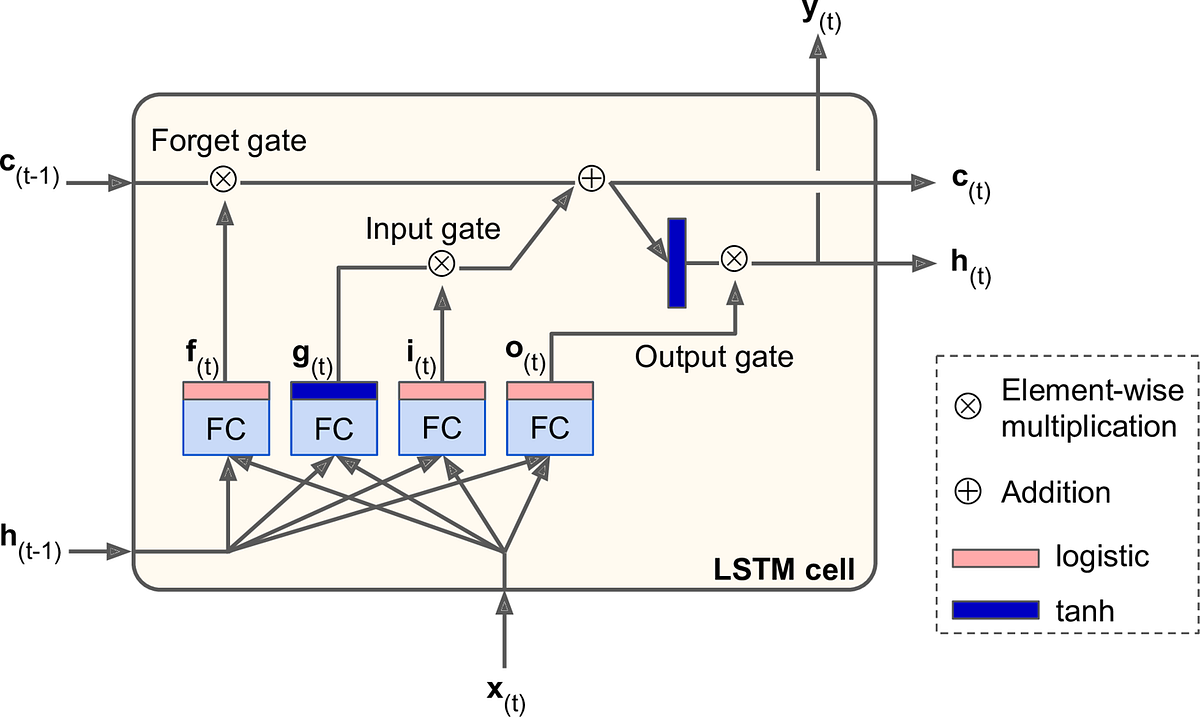
\includegraphics[width=0.85\textwidth]{images/lstm_state_output.png}
    \end{column}
    
    \begin{column}{0.42\textwidth}
      \begin{block}{Обновление ячейки}
        \[
          C_t = f_t \odot C_{t-1} + i_t \odot \tilde{C}_t
        \]
      \end{block}
      
      \begin{block}{Скрытое состояние}
        \[
          h_t = o_t \odot \tanh(C_t)
        \]
      \end{block}
      
      \begin{exampleblock}{Преимущество}
        Градиент протекает через $C_t$.
      \end{exampleblock}
    \end{column}
  \end{columns}
\end{frame}

% Слайд 13: Введение в GRU
\begin{frame}{Gated Recurrent Unit (GRU)}
  \begin{columns}[T]
    \begin{column}{0.45\textwidth}
      \begin{block}{Преимущества}
        \begin{itemize}
          \item Меньше параметров
          \item Быстрее обучение
          \item Меньше переобучение
        \end{itemize}
      \end{block}
      
      \vspace{0.2cm}
      
      \begin{block}{Компоненты}
        \textbf{Два вентиля:}
        \begin{enumerate}
          \item Update ($z_t$)
          \item Reset ($r_t$)
        \end{enumerate}
        
        \textbf{Единое состояние:} $h_t$       \end{block}
    \end{column}
    
    \begin{column}{0.45\textwidth}
      \begin{block}{Сравнение}
        \centering
        \small
        \begin{tabular}{lcc}
          \toprule
          & \textbf{LSTM} & \textbf{GRU} \\
          \midrule
          Вентили & 3 & 2 \\
          Парам. & Больше & Меньше \\
          Скорость & Медл. & Быстр. \\
          \bottomrule
        \end{tabular}
      \end{block}
    \end{column}
  \end{columns}
\end{frame}

% Слайд 14: Математика GRU
\begin{frame}{Математика GRU}
  \begin{block}{Reset Gate}
    \[
      r_t = \sigma(W_r [h_{t-1}, x_t])
    \]
  \end{block}
  
  \begin{block}{Update Gate}
    \[
      z_t = \sigma(W_z [h_{t-1}, x_t])
    \]
  \end{block}
  
  \begin{block}{Обновление состояния}
    \[
      h_t = (1 - z_t) \odot h_{t-1} + z_t \odot \tilde{h}_t, \quad \tilde{h}_t = \tanh(W [r_t \odot h_{t-1}, x_t])
    \]
  \end{block}
\end{frame}

% Слайд 15: Сравнение архитектур
\begin{frame}{Сравнение архитектур}
  \begin{block}{Сравнительная таблица}
    \centering
    \scriptsize
    \begin{tabular}{lccc}
      \toprule
      \textbf{Характ.} & \textbf{Vanilla} & \textbf{LSTM} & \textbf{GRU} \\
      \midrule
      Параметры & Мин. & Макс. & Средн. \\
      Скорость & Быстро & Медл. & Быстро \\
      Память & Плохо & Отлично & Хорошо \\
      Градиент & Проблема & Решена & Решена \\
      Сложность & Низк. & Выс. & Средн. \\
      \bottomrule
    \end{tabular}
  \end{block}
  
  \vspace{0.2cm}
  
  \begin{columns}[T]
    \begin{column}{0.3\textwidth}
      \begin{alertblock}{Vanilla}
        \scriptsize
        Академический интерес, редко на практике
      \end{alertblock}
    \end{column}
    
    \begin{column}{0.3\textwidth}
      \begin{block}{LSTM}
        \scriptsize
        Стандарт для сложных задач
      \end{block}
    \end{column}
    
    \begin{column}{0.3\textwidth}
      \begin{exampleblock}{GRU}
        \scriptsize
        Баланс качества и скорости
      \end{exampleblock}
    \end{column}
  \end{columns}
\end{frame}

% Слайд 16: Применение в NLP
\begin{frame}{Применение в NLP}
  \begin{columns}[T]
    \begin{column}{0.3\textwidth}
      \begin{block}{Тональность}
        \scriptsize
        \textbf{Many-to-One}
        \begin{itemize}
          \item "Love" $\to$ POS
          \item "Bad" $\to$ NEG
        \end{itemize}
      \end{block}
    \end{column}
    
    \begin{column}{0.3\textwidth}
      \begin{block}{Перевод}
        \scriptsize
        \textbf{Seq2Seq}
        \begin{enumerate}
          \item Encoder
          \item Context
          \item Decoder
        \end{enumerate}
      \end{block}
    \end{column}
    
    \begin{column}{0.3\textwidth}
      \begin{block}{Генерация}
        \scriptsize
        \textbf{Language Models}
        \begin{itemize}
          \item Следующее слово
          \item Чат-боты
        \end{itemize}
      \end{block}
    \end{column}
  \end{columns}
\end{frame}

% Слайд 17: Временные ряды и речь
\begin{frame}{Временные ряды и Речь}
  \begin{columns}[T]
    \begin{column}{0.3\textwidth}
      \begin{block}{Прогнозирование}
        \scriptsize
        \begin{itemize}
          \item Цены акций
          \item Погода
          \item Нагрузка
        \end{itemize}
        \textbf{Many-to-Many}
      \end{block}
    \end{column}
    
    \begin{column}{0.3\textwidth}
      \begin{block}{Распознавание речи}
        \scriptsize
        Аудио $\to$ Текст
        \begin{itemize}
          \item Ассистенты
          \item Субтитры
        \end{itemize}
      \end{block}
    \end{column}
    
    \begin{column}{0.3\textwidth}
      \begin{block}{Музыка}
        \scriptsize
        \textbf{Many-to-Many}
        \begin{itemize}
          \item WaveNet
          \item Music Trans.
        \end{itemize}
      \end{block}
    \end{column}
  \end{columns}
\end{frame}

% Слайд 18: Продвинутые архитектуры
\begin{frame}{Продвинутые архитектуры}
  \begin{columns}[T]
    \begin{column}{0.3\textwidth}
      \begin{block}{Bidirectional}
        \scriptsize
        Оба направления:
        \begin{itemize}
          \item Forward
          \item Backward
          \item Concat
        \end{itemize}
      \end{block}
    \end{column}
    
    \begin{column}{0.3\textwidth}
      \begin{block}{Deep RNN}
        \scriptsize
        Несколько слоев:
        \begin{itemize}
          \item Иерархия
          \item Сложн. признаки
        \end{itemize}
      \end{block}
    \end{column}
    
    \begin{column}{0.3\textwidth}
      \begin{block}{Attention}
        \scriptsize
        Важные части:
        \begin{itemize}
          \item Веса $\alpha_i$           \item Контекст
        \end{itemize}
        $\to$ Transformers
      \end{block}
    \end{column}
  \end{columns}
\end{frame}

% Слайд 19: Ограничения и современные тенденции
\begin{frame}{Ограничения и современные тенденции}
  \begin{columns}[T]
    \begin{column}{0.45\textwidth}
      \begin{alertblock}{Ограничения}
        \scriptsize
        \begin{enumerate}
          \item \textbf{Последовательность}
            \begin{itemize}
              \item Без распараллеливания
              \item Медленное обучение
            \end{itemize}
          
          \item \textbf{Контекст}
            \begin{itemize}
              \item Теряют память
            \end{itemize}
        \end{enumerate}
      \end{alertblock}
    \end{column}
    
    \begin{column}{0.45\textwidth}
      \begin{exampleblock}{Тенденции}
        \scriptsize
        \textbf{Transformers:}
        \begin{itemize}
          \item Распараллеливание
          \item Self-Attention
        \end{itemize}
        
        \textbf{Модели:} BERT, GPT
        
        \textbf{Где RNN полезны:}
        \begin{itemize}
          \item Stream
          \item Edge
          \item Real-time
        \end{itemize}
      \end{exampleblock}
    \end{column}
  \end{columns}
\end{frame}

% Слайд 20: Заключение
\begin{frame}{Заключение}
  \begin{block}{Ключевые выводы}
    \scriptsize
    \begin{enumerate}
      \item \textbf{RNN} ввели память в нейронные сети
      
      \item \textbf{LSTM, GRU} решили проблему градиентов
      
      \item \textbf{Attention} → Transformers
      
      \item RNN заложили основы последовательных моделей
    \end{enumerate}
  \end{block}
  
  \vspace{0.2cm}
  
  \begin{exampleblock}{Будущее}
    \scriptsize
    Принципы RNN остаются важными:
    \begin{itemize}
      \item Последовательные данные
      \item Механизмы внимания
      \item Баланс память/вычисления
    \end{itemize}
  \end{exampleblock}
  
  \centering
  \vspace{0.2cm}
  {\small \textbf{Спасибо за внимание!}}
\end{frame}

\end{document}